\chapter{Resultados e Discussão}
%TODO: Inserir Introdução ao capítulo.

\section{Validação Computacional (Simulação)}
%TODO? Falar sobre a modelagem dos capacitores da simulação?

Para a validação conceitual do hardware de potência antes da montagem física, utilizou-se o software \textbf{LTSpice}. A simulação concentrou-se no estágio de potência do inversor, modelando as chaves semicondutoras e a carga indutiva. Foram elaborados dois cenários de simulação: uma topologia monofásica (meia-ponte) para análise isolada e uma topologia trifásica completa para validação do fluxo de corrente inter-fases (Figura \ref{fig:simulacao_trifasica}).

\begin{figure}[H]
    \centering
    \caption{Esquemático da simulação trifásica do ESC em estado estático de comutação.}
    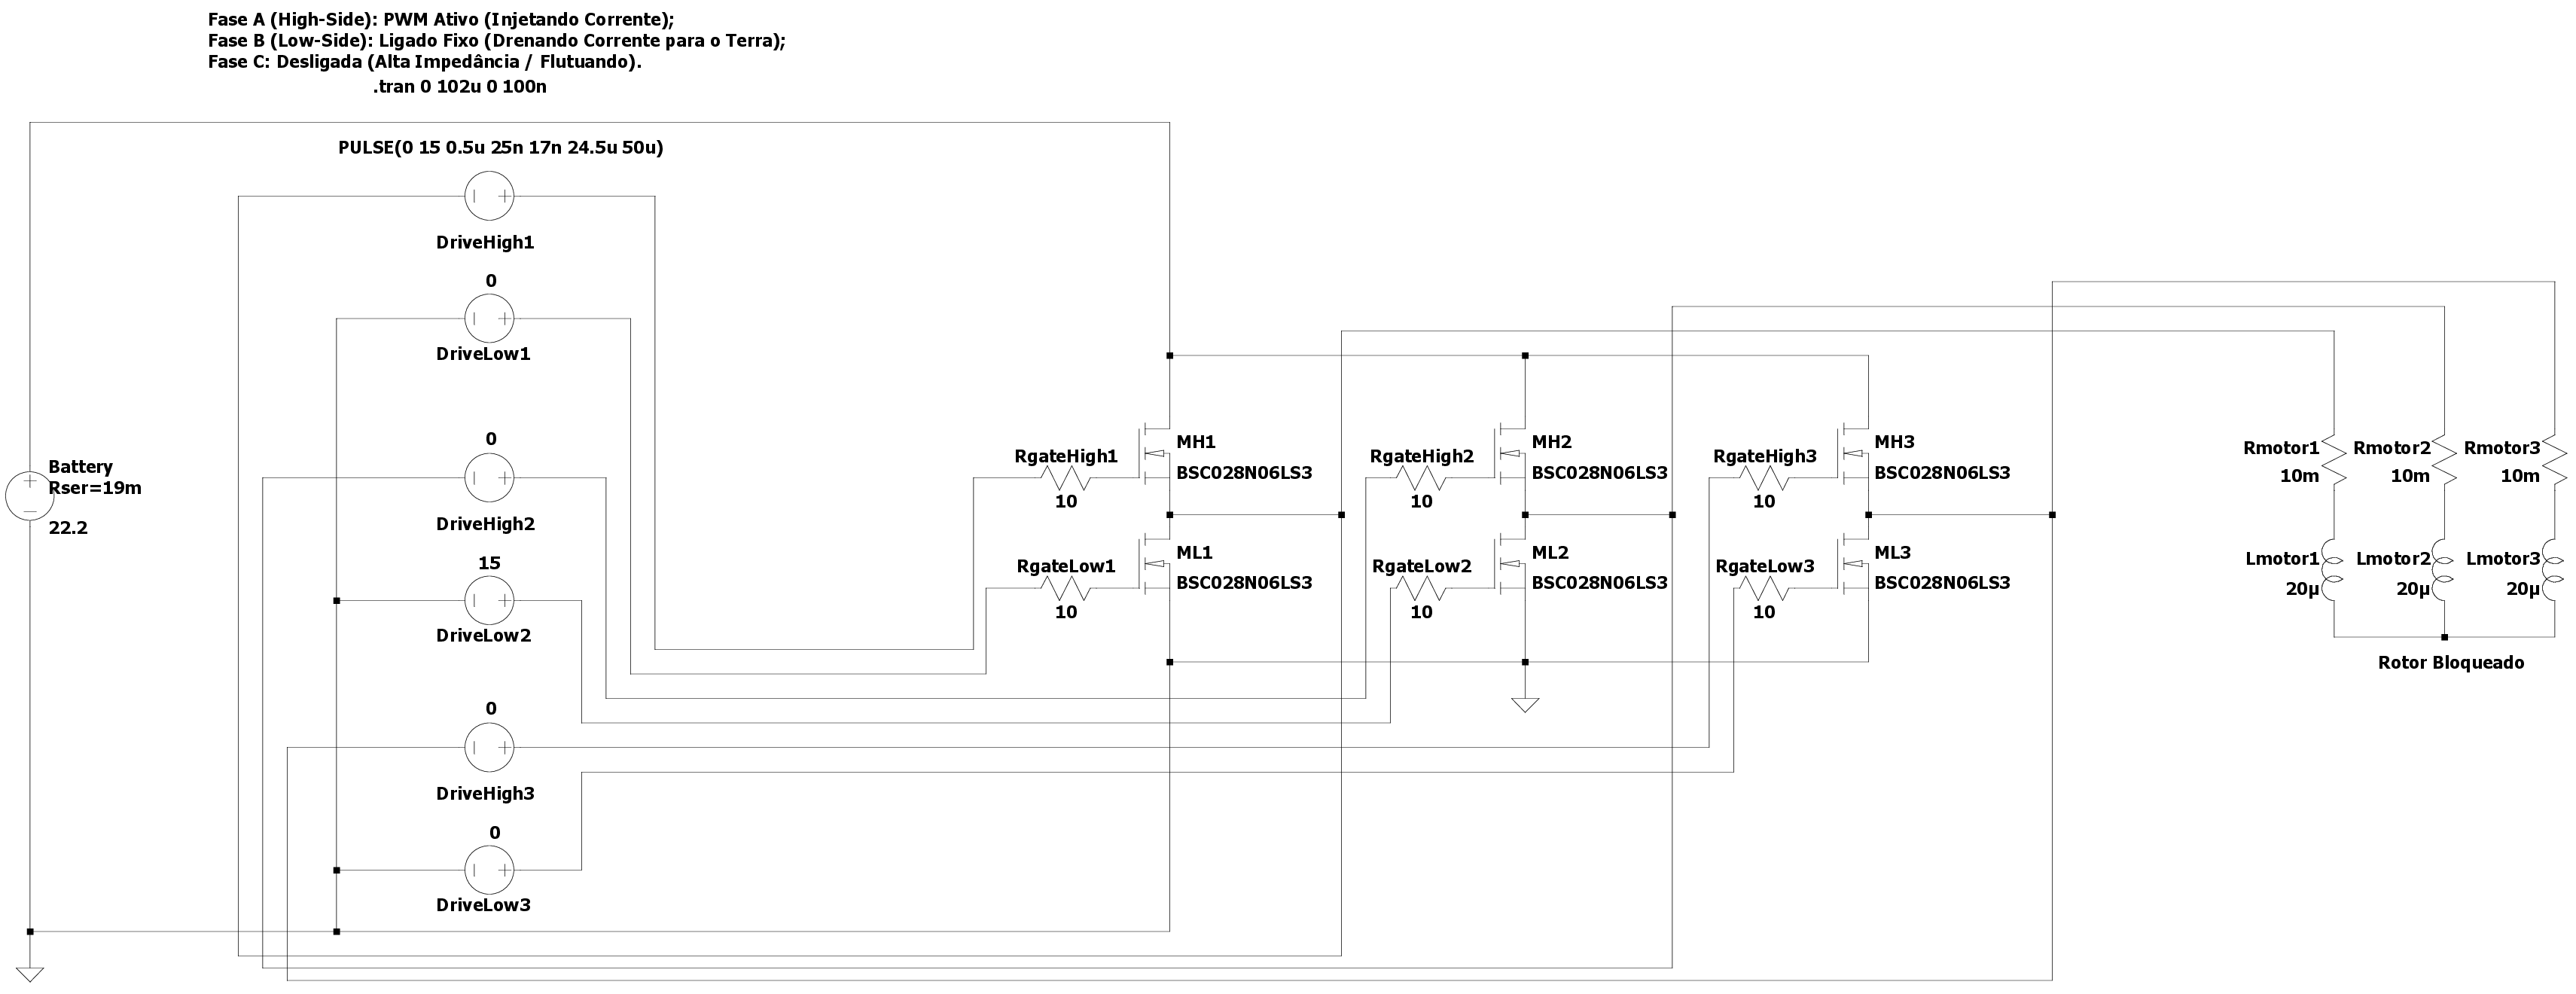
\includegraphics[width=17cm]{Simulation/trifasico.png}
    \caption*{Fonte: Elaborado pelo autor.}
    \label{fig:simulacao_trifasica}
\end{figure}

O circuito é dividido em três blocos funcionais: alimentação, comutação e carga. A fonte de energia primária é modelada por uma fonte DC de $22,2 \: V$ com uma resistência série ($R_{ser}$) de $19 \: m\Omega$, emulando com precisão a dinâmica de descarga e as perdas ôhmicas internas da bateria LiPo 6S definida para o projeto. O estágio de comutação é composto por uma ponte inversora trifásica utilizando transistores MOSFET (modelo comportamental BSC028N06LS3). As portas (\textit{gates}) destes semicondutores são excitadas através de resistores de $10 \: \Omega$, valor projetado para limitar a corrente de pico do \textit{driver} e amortecer ressonâncias (\textit{ringing}) parasitas sem degradar o tempo de comutação. O acionamento através dos \textbf{drivers de gate} foram modeladas utilizando fontes de tensão do tipo pulso. O sinal de acionamento do lado alto (\textit{High-Side}) da Fase A foi definido com os parâmetros \texttt{PULSE(0 15 0 100n 100n 25u 50u)}, forçando a condução do Passo 1 da sequência trapezoidal. Este perfil injeta um sinal com amplitude de $15\text{V}$, estabelecendo uma frequência de chaveamento de \textbf{$20\text{ kHz}$} (período de $50 \mu\text{s}$) e um ciclo de trabalho (\textit{Duty Cycle}) de \textbf{$50\%$}. Os tempos de transição de subida e descida foram definidos em $100\text{ ns}$ para simular o tempo de resposta do gate do \textbf{MOSFET}.

Por fim, o motor BLDC é representado por seu modelo elétrico equivalente de estator, consistindo em três ramos conectados em estrela (neutro comum). Cada fase possui uma resistência de armadura corrigida de $10 \: m\Omega$ em série com uma indutância de $20 \: \mu H$. Esta modelagem a rotor bloqueado força o sistema a operar sob a condição mais severa de estresse elétrico, permitindo avaliar a capacidade máxima de condução de corrente dos transistores e a resposta transitória da rede indutiva sem a oposição da Força Contraeletromotriz (FCEM), garantindo que os resultados da simulação representem o limite operacional do \textit{hardware}. 

Como o esquemático foca na validação da transferência de energia em um instante específico da \textbf{comutação de seis passos} (Fase A injetando corrente e Fase B drenando para o terra), o transistor do lado baixo da Fase A foi mantido em \textbf{corte} ($0\text{V}$ constante). Devido a esta modelagem estática de um único passo, a inserção de um \textbf{tempo morto ($t_{dead}$)} dinâmico não se fez necessária no gerador de pulsos, assumindo-se o isolamento ideal entre os estados de condução. O motor foi adequadamente modelado na condição de \textbf{rotor bloqueado}, respeitando os parâmetros intrínsecos de resistência ($R = 10m \Omega$) e indutância ($L = 20 \mu\text{H}$) por fase.

A Figura \ref{fig:sim_correntes_motor} apresenta os resultados transitórios das correntes de fase ($I_A$, $I_B$ e $I_C$) durante os dois primeiros ciclos de chaveamento do inversor, totalizando $100 \: \mu s$. Observa-se que, durante o primeiro tempo de condução ($T_{on}$) do sinal PWM entre $0$ e $25 \: \mu s$, a corrente $I_A$ ascende de forma linear até atingir o patamar de aproximadamente $13,5 \: A$. Simultaneamente, a corrente $I_B$ apresenta a mesma magnitude, porém com polaridade invertida ($-13,5 \: A$), enquanto a corrente $I_C$ permanece nula, oscilando apenas com os ruídos numéricos do simulador próximos a zero. Durante o tempo de bloqueio do PWM ($T_{off}$) entre $25 \: \mu s$ e $50 \: \mu s$, as correntes $I_A$ e $I_B$ não caem abruptamente para zero, mas sim sofrem um decaimento suave. O ciclo se repete aos $50 \: \mu s$, elevando as correntes ao patamar de $26 \: A$.

\begin{figure}[H]
    \centering
    \caption{Dinâmica das correntes de fase do motor durante os primeiros $100 \: \mu s$ de simulação (Passo 1).}
    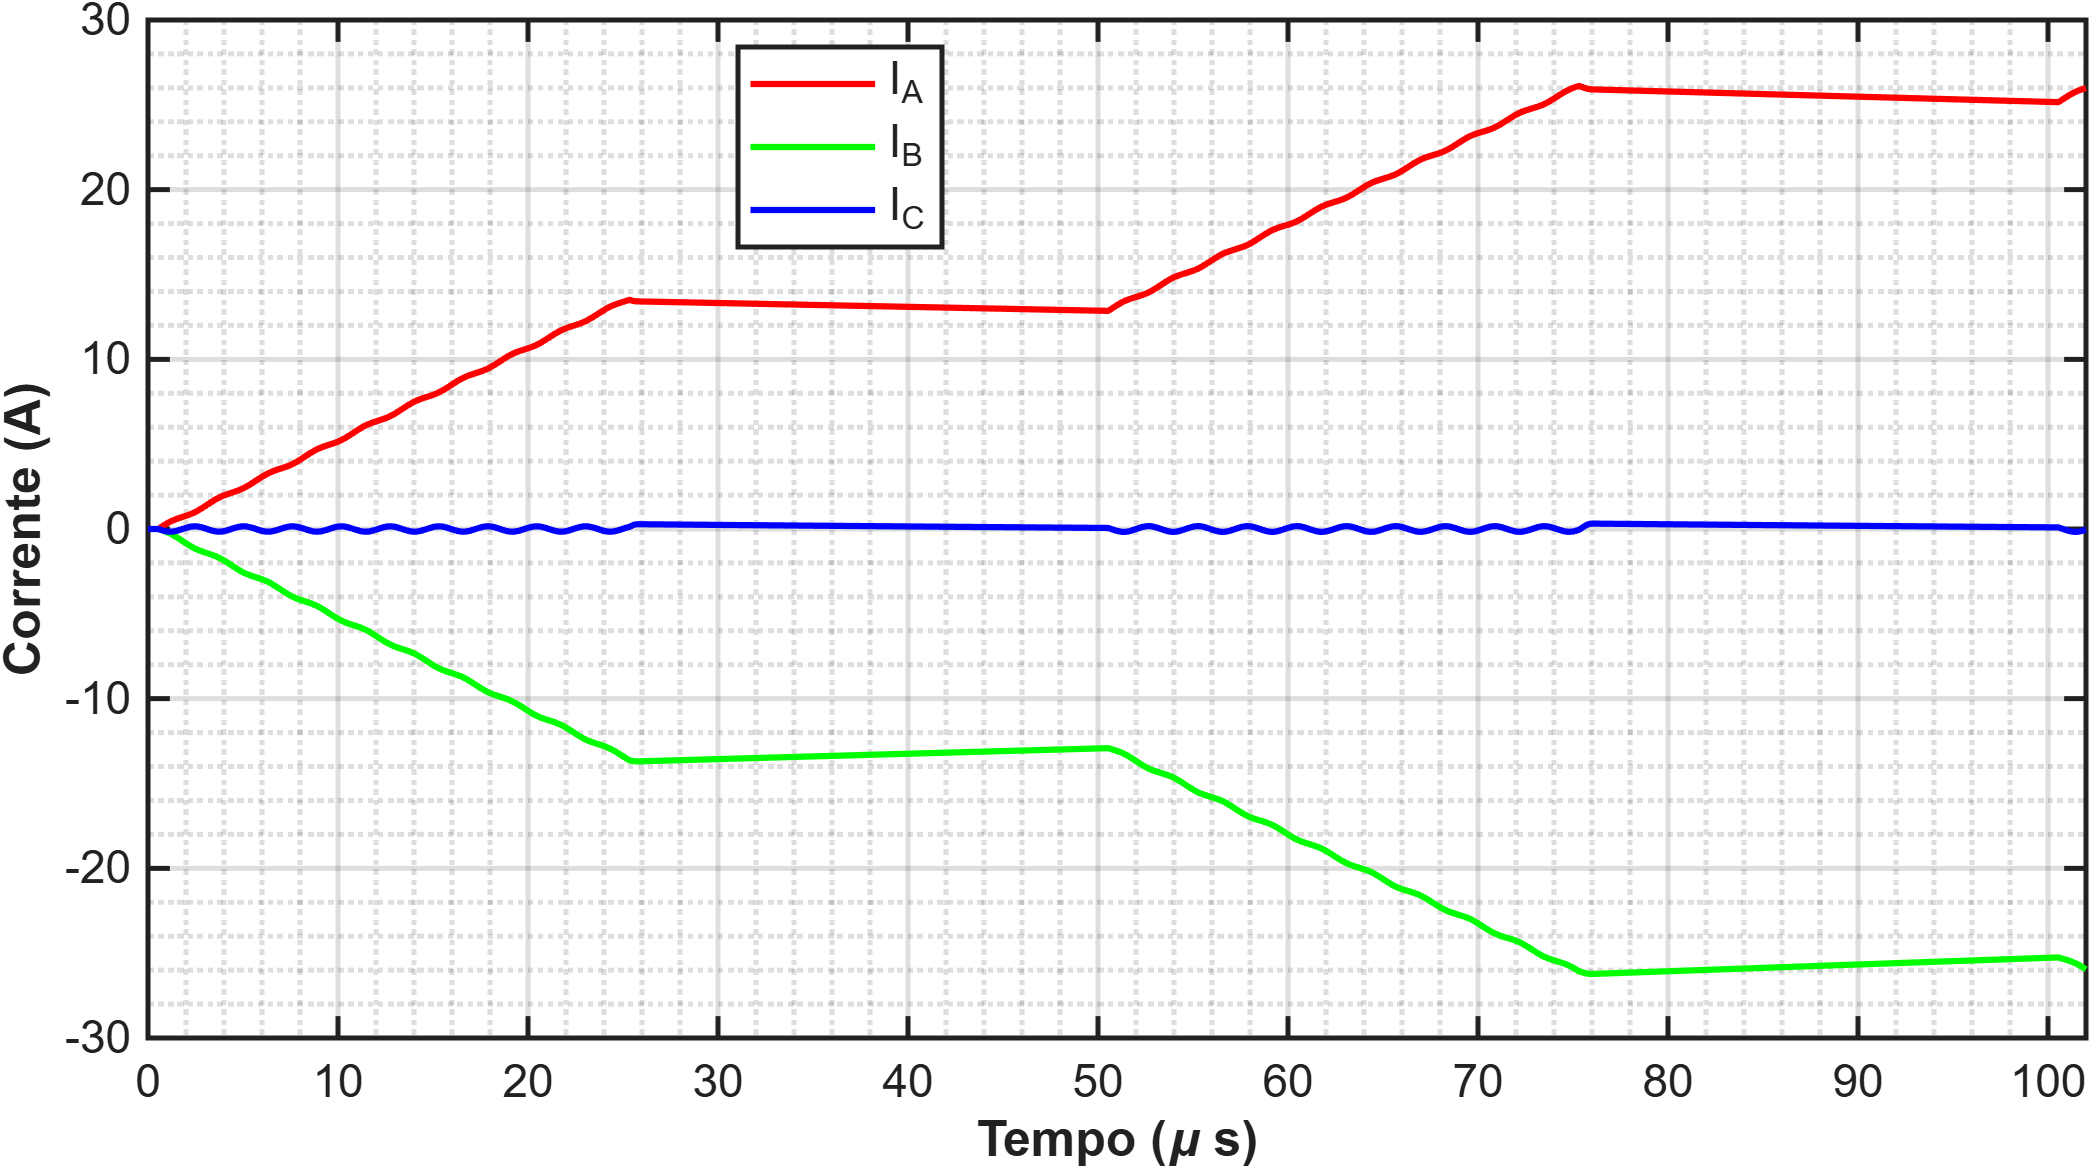
\includegraphics[width=0.8\textwidth]{Simulation/plot_simulacao/1_correntes_motor.png}
    \caption*{Fonte: Elaborado pelo autor.}
    \label{fig:sim_correntes_motor}
\end{figure}

Este comportamento é a resposta direta da excitação do circuito indutivo do estator sob a topologia de modulação \textit{High-Side PWM / Low-Side ON}. Ao disparar o transistor superior da fase A e manter o transistor inferior da fase B em condução plena, estabelece-se um fluxo de elétrons que obrigatoriamente passa por duas bobinas em série ($V = L_{eq} \frac{di}{dt} + R_{eq}i$). A inclinação constante ($di/dt$) da rampa de corrente é ditada pela reatância indutiva nominal do motor. Durante o ciclo $T_{off}$ da chave superior, a energia magnética armazenada na indutância do estator força a manutenção do fluxo de corrente, que encontra caminho através do diodo de roda livre (\textit{freewheeling diodo}) intrínseco ao MOSFET inferior da fase A, justificando a lenta taxa de decaimento observada.

Ao compararmos com o arcabouço teórico, o resultado valida a comutação de seis passos apresentada na Tabela \ref{tab:mcpwm_map}. A frequência estabelecida pelo projeto de $20 \: kHz$ é ratificada pelo período exato de $50 \: \mu s$ entre os picos de chaveamento. Mais importante ainda, a completa inércia da fase C ($I_C \approx 0 \: A$) confirma a eficácia do estado de alta impedância (Hi-Z) no braço inversor não excitado, condição \textit{sine qua non} para a medição livre de distorções da Força Contraeletromotriz (FCEM) na posterior transição para a malha fechada.

A Figura \ref{fig:sim_tensoes_neutro} ilustra o comportamento dinâmico das tensões de fase referenciadas ao ponto neutro da carga ($V_{AN}$, $V_{BN}$ e $V_{CN}$). Durante o período de condução do PWM ($T_{on}$), nota-se que o eixo de oscilação das tensões se estabelece em médias de $+11,1 \: V$ para a fase A, $-11,1 \: V$ para a fase B, e $0 \: V$ para a fase C. A severa oscilação de alta frequência (\textit{ringing}) sobreposta aos sinais é um artefato numérico característico do ambiente de simulação. Como a fase C está em estado de alta impedância (flutuante) e o modelo utiliza indutores puros, forma-se um tanque LC não amortecido com as capacitâncias parasitas do transistor, fenômeno que no circuito físico real seria drasticamente atenuado pelas perdas no núcleo ferromagnético do motor e pelo filtro RC do circuito de leitura.

\begin{figure}[H]
    \centering
    \caption{Tensões de fase em relação ao ponto neutro do motor durante o Passo 1.}
    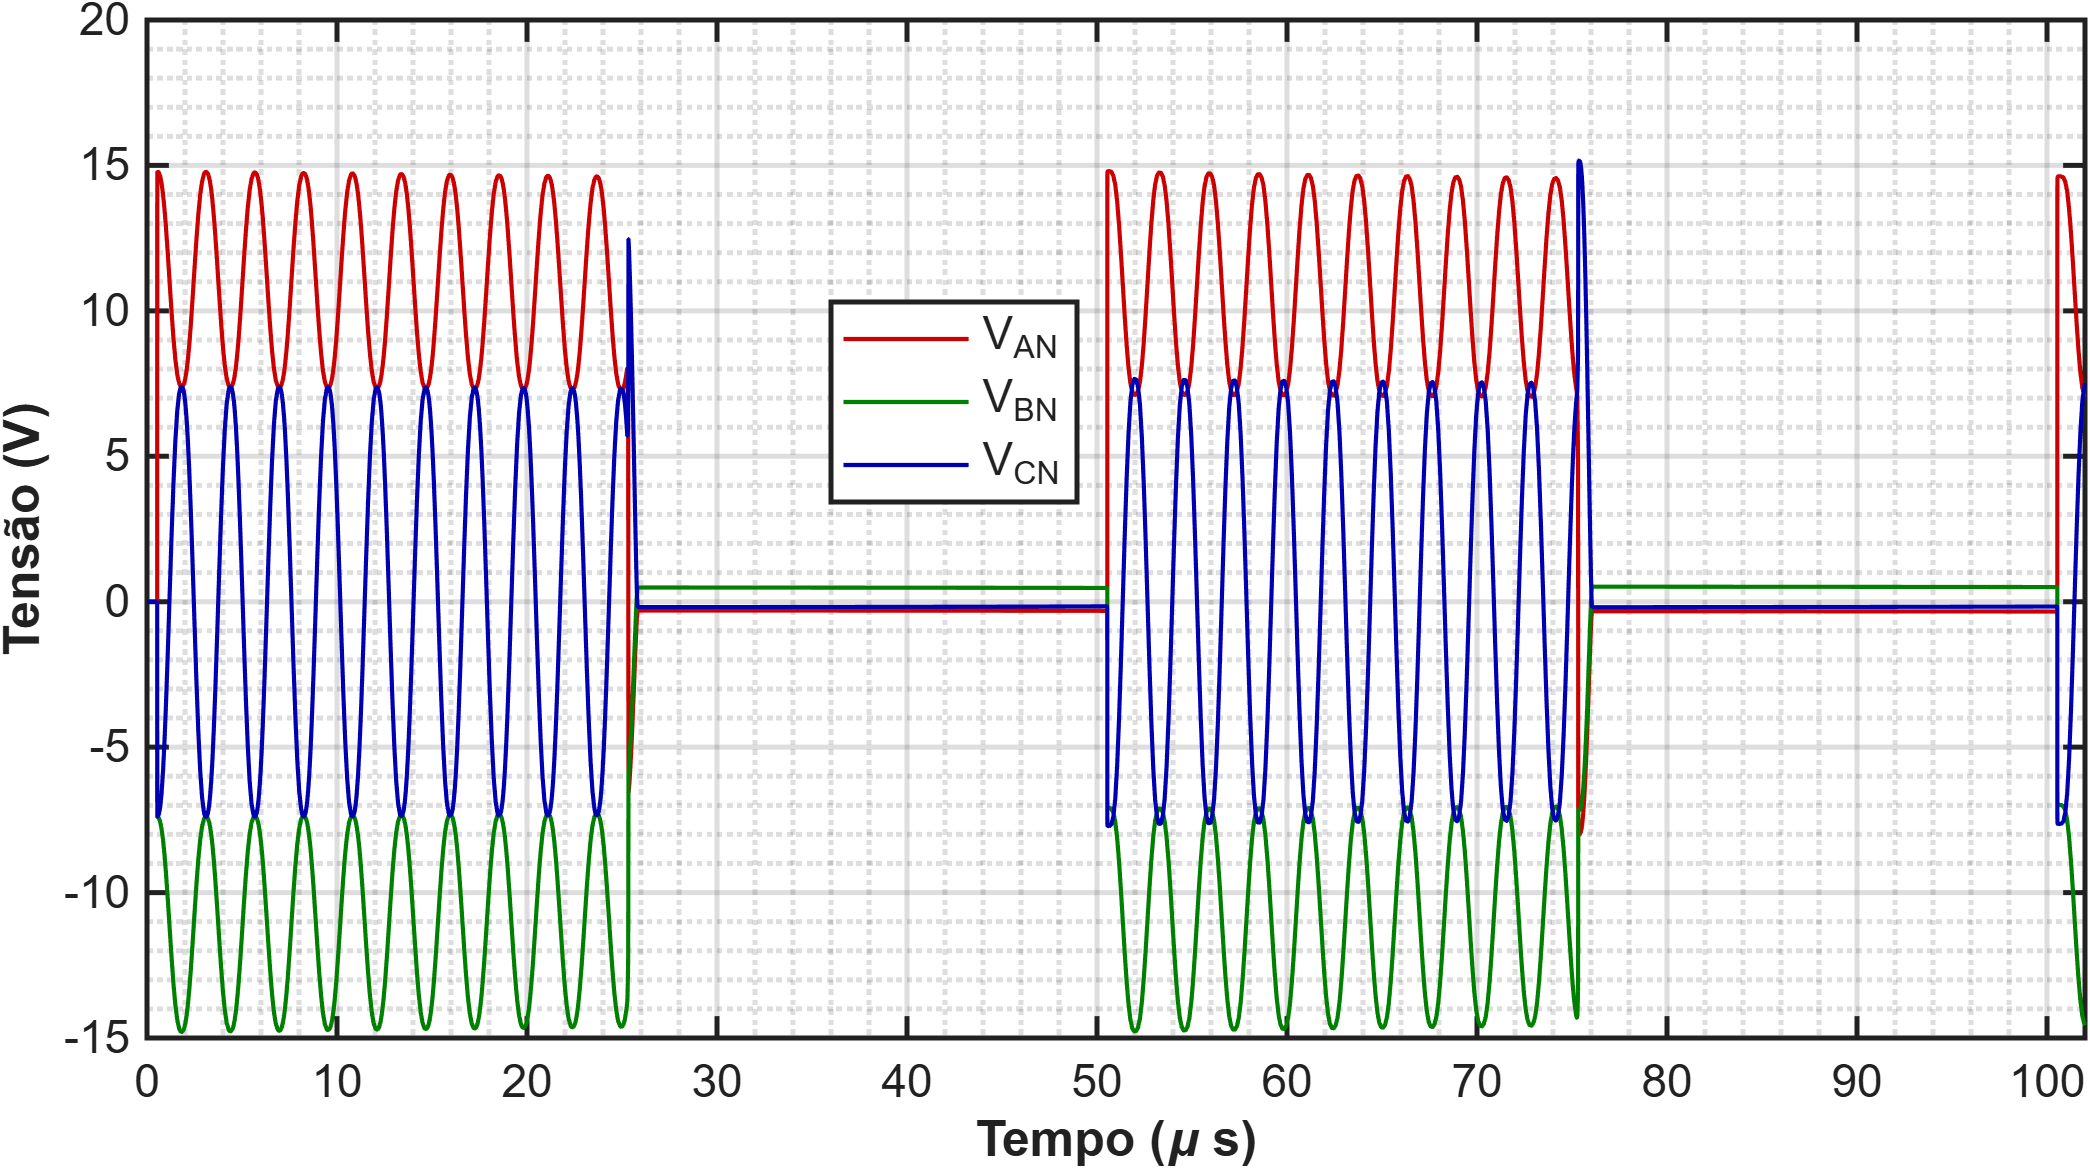
\includegraphics[width=0.8\textwidth]{Simulation/plot_simulacao/3_tensoes_fase_neutro.png}
    \caption*{Fonte: Elaborado pelo autor.}
    \label{fig:sim_tensoes_neutro}
\end{figure}


Do ponto de vista físico, o estabelecimento das tensões em $\pm 11,1 \: V$ é o resultado direto da divisão de potencial no fechamento em estrela (Y) do estator. Com a fase A submetida à tensão plena do barramento ($V_{DC} = 22,2 \: V$) e a fase B conectada ao referencial zero ($0 \: V$), o nó central (neutro) assume naturalmente o potencial médio exato de $11,1 \: V$. Ensaios paralelos nas Fases B e C confirmaram a manutenção do transístor inferior em condução plena ($15 \: V$) e os transistores da fase flutuante em corte ($0 \: V$), atestando a robustez da topologia contra disparos espúrios.

Comparando este resultado com os fundamentos da comutação trapezoidal detalhados na metodologia, a simulação valida a correta formação e estabilidade do potencial de neutro. Esta validação teórica prévia é de suma importância, pois ratifica a viabilidade da técnica de reconstrução de neutro virtual adotada no \textit{hardware}, assegurando que o microcontrolador possuirá uma referência de tensão simétrica e confiável para a detecção da Força Contraeletromotriz (FCEM) durante a operação em malha fechada.

A Figura \ref{fig:sim_bateria_esforco} demonstra o severo esforço transitório imposto à fonte de alimentação primária (bateria LiPo) quando conectada diretamente à ponte inversora, sem o auxílio de capacitores de barramento (\textit{Link DC}), o qual será inserido no projeto final. Observa-se como fato primário que, durante o \textbf{tempo de condução ($T_{on}$)}, a tensão da bateria decai gradualmente de $22,2 \: V$ para aproximadamente $21,9 \: V$, conforme ilustrado na Figura \ref{fig:bateria_tensao}. Esse comportamento acompanha a rampa de subida da corrente, que atinge o patamar de $13 \: A$. O fator mais crítico, no entanto, ocorre nos instantes exatos de comutação ($50 \: \mu s$ e $100 \: \mu s$), nos quais a corrente drena picos agudos que ultrapassam os $130 \: A$ e $200 \: A$, respectivamente, como detalhado na Figura \ref{fig:bateria_corrente}. Esses picos provocam quedas instantâneas (\textit{voltage sags}) severas na tensão da bateria, reduzindo-a para níveis próximos de $19,5 \: V$. Durante o \textbf{tempo de bloqueio ($T_{off}$)}, a corrente da bateria cessa completamente, pois a corrente do motor passa a circular em roda livre pelos diodos da ponte.

\begin{figure}[H]
    \centering
    \caption{Análise dinâmica dos parâmetros de entrada da bateria LiPo no Passo 1 sem filtragem capacitiva: (a) Transiente de tensão; (b) Transiente de corrente.}
    \label{fig:sim_bateria_esforco}
    \begin{subfigure}[b]{0.49\textwidth}
        \centering
        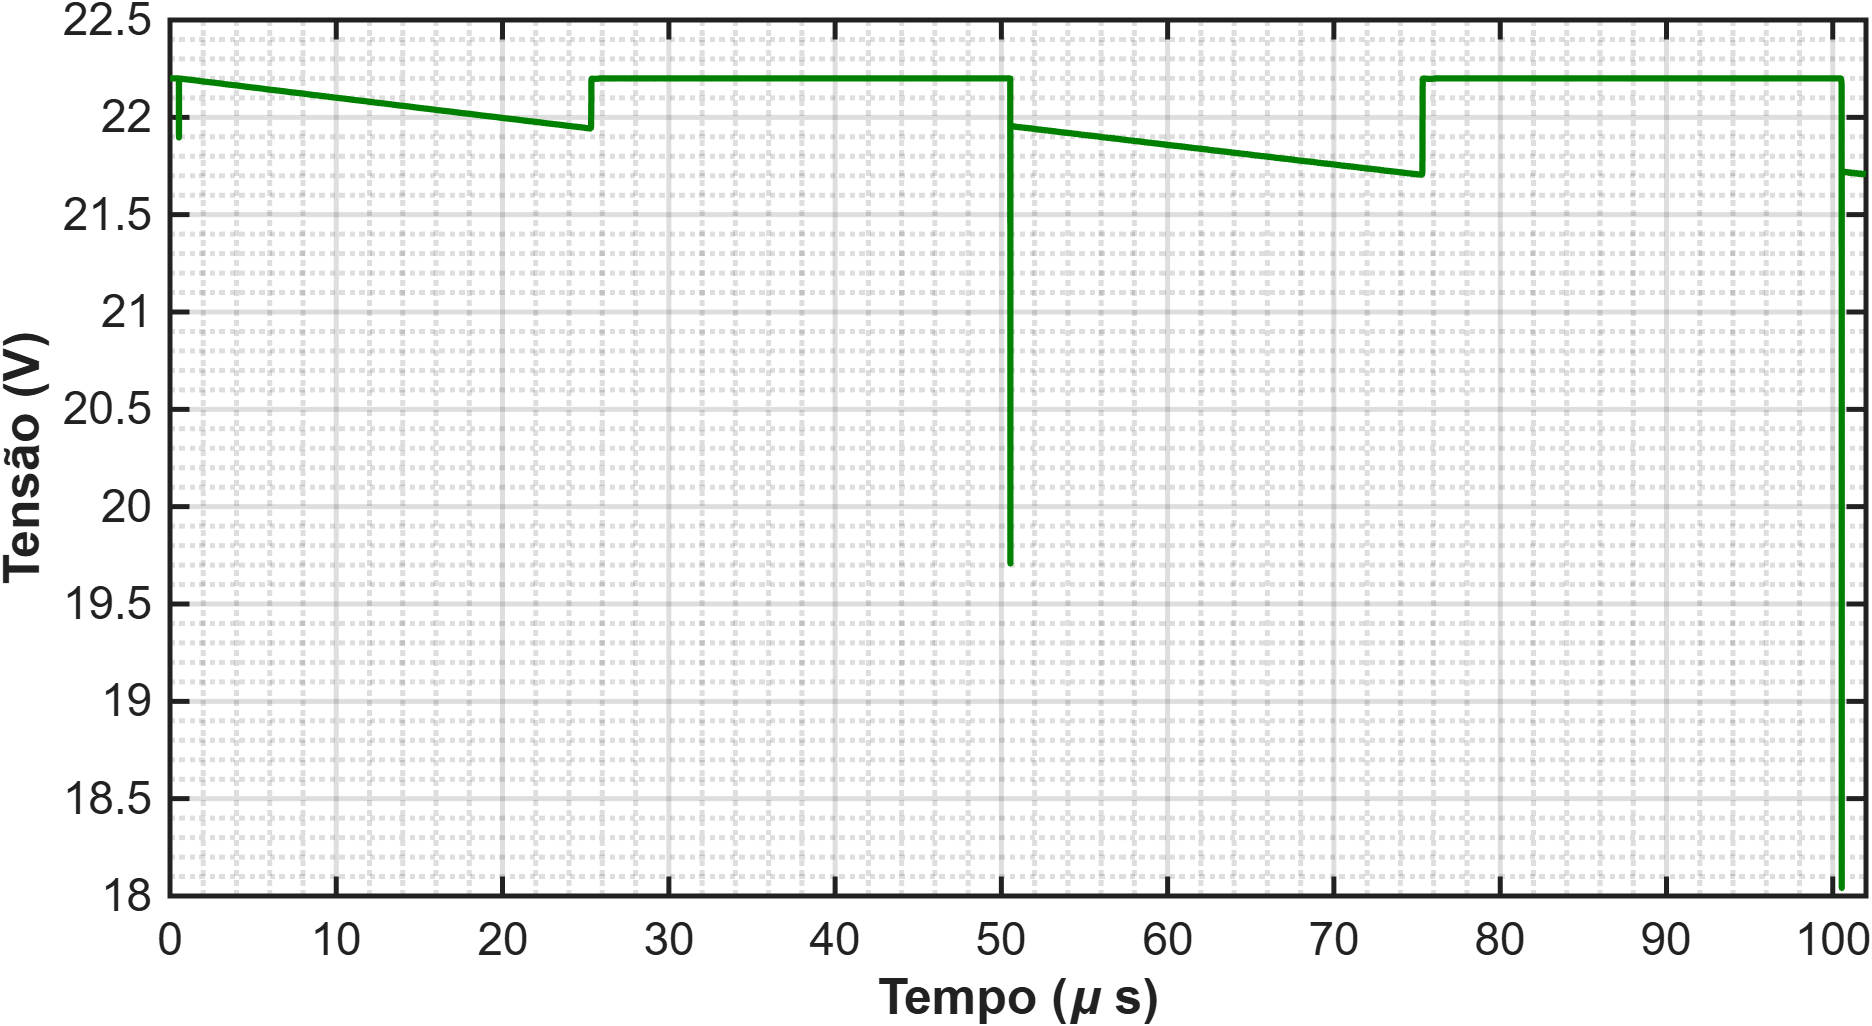
\includegraphics[width=\textwidth]{Simulation/plot_simulacao/7a_bateria_tensao.png}
        \caption{Tensão de barramento.}
        \label{fig:bateria_tensao}
    \end{subfigure}
    \hfill
    \begin{subfigure}[b]{0.49\textwidth}
        \centering
        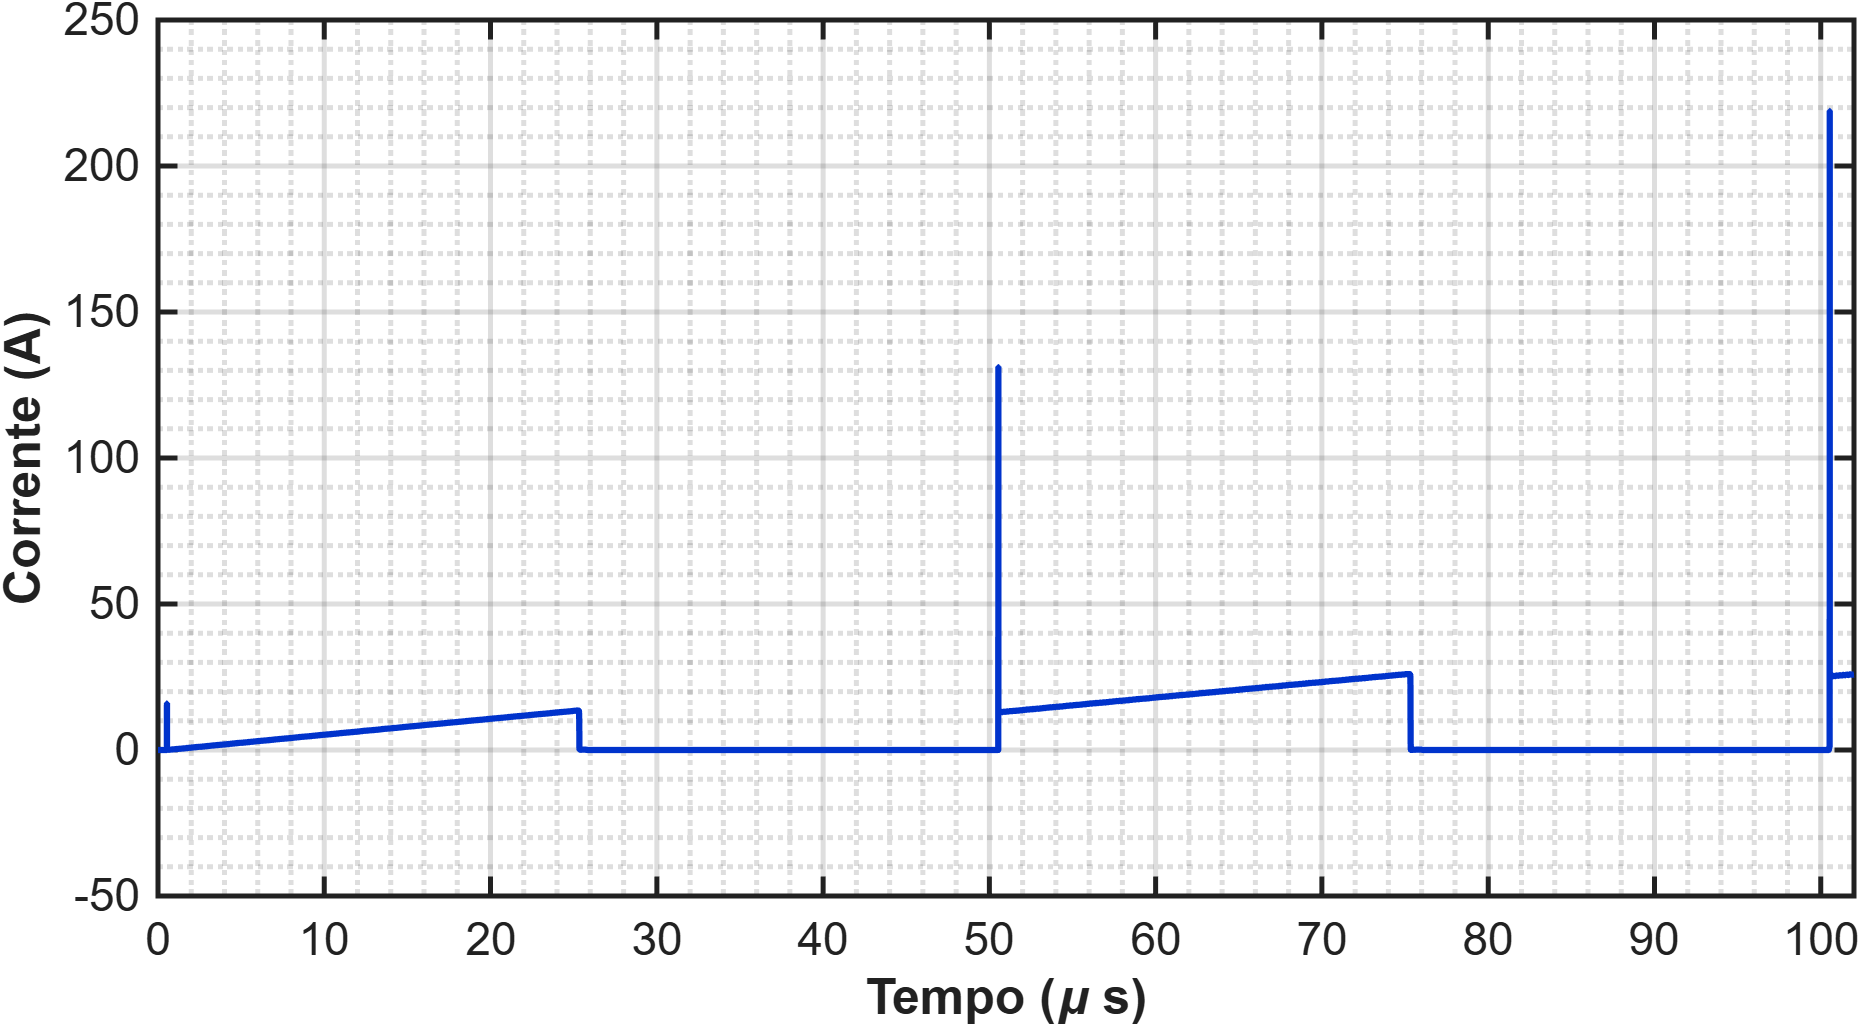
\includegraphics[width=\textwidth]{Simulation/plot_simulacao/7b_bateria_corrente.png}
        \caption{Corrente drenada.}
        \label{fig:bateria_corrente}
    \end{subfigure}
    \caption*{Fonte: Elaborado pelo autor.}
\end{figure}

A causa física para o decaimento gradual da tensão é a queda de potencial ôhmica intrínseca ($V_{drop} = I_a \cdot R_{ser}$) sobre a \textbf{resistência série equivalente} da bateria, que no modelo foi parametrizada como $19 \: m\Omega$. Por outro lado, os transientes agudos (\textit{spikes}) de corrente são consequência da elevadíssima taxa de variação ($di/dt$) exigida para carregar as capacitâncias parasitas dos MOSFETs e suprir a corrente de recuperação reversa (\textit{reverse recovery}) dos diodos corporais nos instantes de ativação (\textit{turn-on}). Como o circuito simulado neste ensaio possui apenas a bateria como fonte de energia, ela é forçada a fornecer instantaneamente toda a carga transitória.

A comparação deste comportamento simulado com a teoria de eletrônica de potência com o dimensionamento estabelecido na Metodologia. A simulação prova que submeter uma bateria LiPo a este nível de corrente de ondulação (\textit{ripple}) e picos transientes resultaria em superaquecimento severo e degradação química prematura das células. Fica, portanto, validada a necessidade imperativa da instalação do banco de \textbf{capacitores de filtro Low-ESR} ($940 \: \mu F$) projetado fisicamente na placa de circuito impresso (PCB), cuja função será atuar como um reservatório local de energia de baixíssima impedância para absorver estes transientes de alta frequência, isolando e protegendo a fonte primária.

\section{Projeto Eletrônico e Análise dos Esquemáticos}
%TODO: Inserir Introdução do capítulo.

\subsection{Circuito de Alimentação Auxiliar e Regulação}

A Figura \ref{fig:esquematico_supply} detalha a arquitetura de entrada e distribuição de energia do ESC. A conexão primária é realizada através de um conector de alta capacidade XT90, protegida imediatamente em série por um \textbf{fusível MIDI} de $80 \: A$ (modelo 0498080.M). O barramento DC (\textit{Link DC}) é suportado por um banco de capacitores híbrido em topologia paralela, composto por seis capacitores polarizados de $220 \: \mu F$ e três capacitores cerâmicos não polarizados de $1 \: \mu F$. A partir deste barramento filtrado, a tensão nominal da bateria alimenta dois módulos conversores \textit{buck} LM2596 dispostos em paralelo, responsáveis por gerar as malhas de tensão independentes de $15 \: V$ (\textit{Vcc 1}) e $5 \: V$ (\textit{Vcc 2}). Adicionalmente, o esquemático implementa uma separação explícita entre o \textbf{terra de potência (PGND)} e o \textbf{terra de sinal (SGND)}, interligados fisicamente por um único componente passivo limitador de laço (RJ1).

\begin{figure}[H]
    \centering
    \caption{Esquemático do estágio de entrada, filtragem do barramento DC e regulação de tensão auxiliar (Folha \textit{Supply}).}
    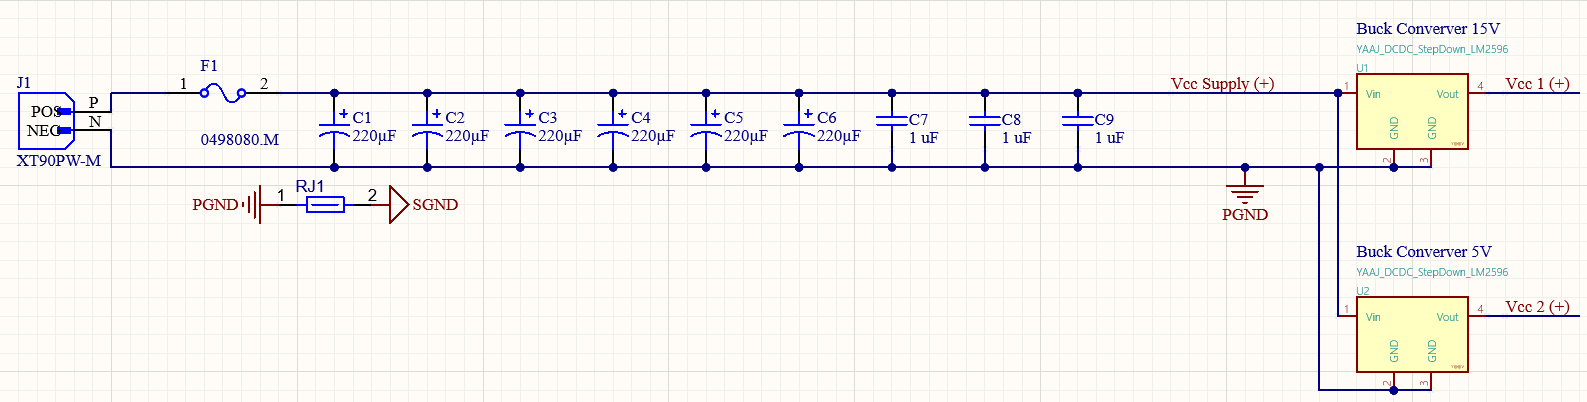
\includegraphics[width=1\textwidth]{imagens/esquematico_supply.png}
    \caption*{Fonte: Elaborado pelo autor.}
    \label{fig:esquematico_supply}
\end{figure}

Fisicamente, a divisão do banco capacitivo em múltiplas unidades de $220 \: \mu F$ reduz drasticamente a \textbf{Resistência Série Equivalente (ESR)} total do barramento, otimizando a absorção da elevada corrente de ondulação (\textit{ripple}) gerada pela ponte inversora sem causar aquecimento excessivo nos componentes. Os capacitores cerâmicos de $1 \: \mu F$ atuam no desacoplamento de alta frequência, suprimindo transientes que os capacitores eletrolíticos não conseguem filtrar devido à sua \textbf{Indutância Série Equivalente (ESL)}. A separação galvânica e o controle de retorno por meio da junção estrita entre \textbf{PGND} e \textbf{SGND} (\textit{Star Grounding}) impedem que as severas correntes de comutação do motor provoquem flutuações de tensão (\textit{ground bounce}) no referencial sensível do microcontrolador. 

A comparação com a metodologia teórica comprova a evolução e a robustez do projeto prático. Enquanto o texto preliminar previa genericamente a filtragem do \textit{Link DC} e reguladores em cascata, o arranjo físico adota conversores LM2596 dispostos em paralelo. Esta decisão elimina o gargalo térmico de fazer o regulador de menor tensão drenar corrente através do regulador primário, garantindo maior eficiência e isolamento entre o circuito de acionamento de \textit{gate} ($15 \: V$) e a lógica de processamento digital ($5 \: V$).

\subsection{Unidade de Processamento Lógico e Interface de Acionamento}

A Figura \ref{fig:esquematico_control} ilustra o núcleo de inteligência do ESC e sua interface direta com o estágio de potência. A Unidade de Processamento, baseada no módulo ESP32 (Figura \ref{fig:control_esp32}), é alimentada pela malha de $5 \: V$ (\textit{Vcc 2}). O regulador linear interno do microcontrolador reduz essa tensão para $3,3 \: V$, sinal que é exportado pelo pino 1 sob a nomenclatura \textit{Vmicro Ref}. Esta estratégia de projeto é fundamental: o \textit{Vmicro Ref} é roteado diretamente para os pinos de alimentação lógica (\textit{VDD}) dos três \textit{drivers} IR2110 (Figura \ref{fig:control_drivers}). Isso garante que o limiar de transição lógica (\textit{logic high threshold}) dos \textit{drivers} seja idêntico à tensão de saída dos pinos GPIO do ESP32, eliminando falhas de interpretação de sinal por incompatibilidade de níveis de tensão.

\begin{figure}[H]
    \centering
    \caption{Esquemáticos do núcleo de controle e interface de potência: (a) Microcontrolador ESP32-WROOM-32; (b) Estágio de translação de nível com \textit{drivers} IR2110.}
    \label{fig:esquematico_control}
    \begin{subfigure}[b]{0.48\textwidth}
        \centering
        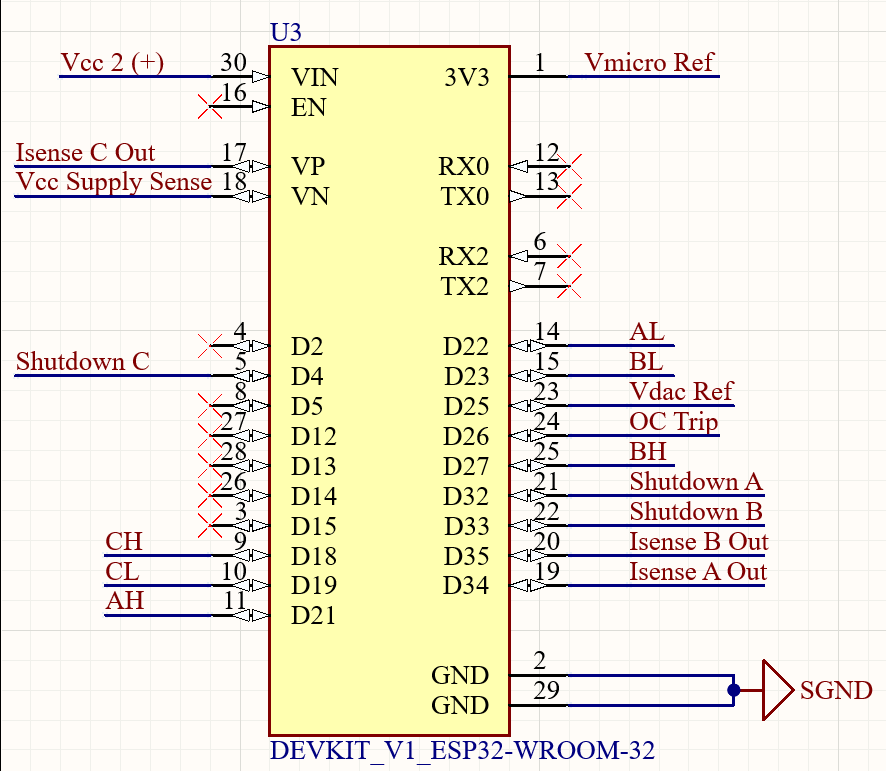
\includegraphics[width=\textwidth]{imagens/esp32_schematic.png}
        \caption{Unidade de Processamento (ESP32).}
        \label{fig:control_esp32}
    \end{subfigure}
    \hfill
    \begin{subfigure}[b]{0.48\textwidth}
        \centering
        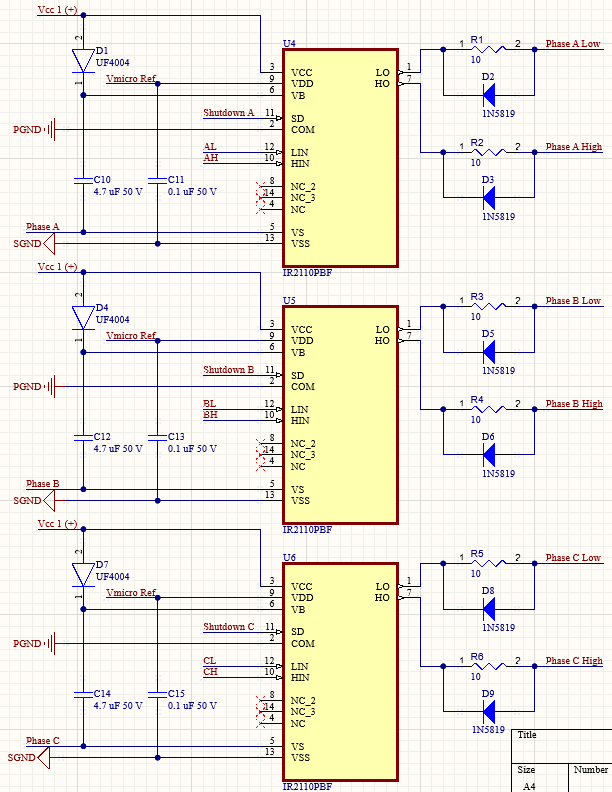
\includegraphics[width=\textwidth]{imagens/ir2110_schematic.png}
        \caption{\textit{Drivers} de \textit{Gate} (IR2110).}
        \label{fig:control_drivers}
    \end{subfigure}
    \caption*{Fonte: Elaborado pelo autor.}
\end{figure}

O isolamento contra ruídos é efetivado pela segregação dos planos de terra nos \textit{drivers} IR2110. O referencial lógico (\textit{VSS}) é conectado exclusivamente ao terra de sinal (\textbf{SGND}), enquanto o retorno de potência (\textit{COM}), que lida com os pulsos de alta corrente de carga e descarga dos MOSFETs, é roteado para o terra de potência (\textbf{PGND}). A comunicação de segurança entre o microcontrolador e os \textit{drivers} ocorre de forma redundante: o ESP32 gera os seis sinais do MCPWM ($AH, AL$, etc.) e possui controle direto sobre os pinos de \textit{Shutdown} ($SD$) de cada IR2110. Adicionalmente, o pino \textit{OC Trip} (\textit{Overcurrent Trip}) permite que um evento de falta detectado pelos sensores interrompa a geração de PWM no \textit{hardware} do ESP32 em microssegundos.

Na saída dos \textit{drivers}, o esquemático valida o projeto do circuito de \textit{bootstrap} e o condicionamento de \textit{gate}. A malha de \textit{bootstrap} utiliza um diodo de recuperação ultra-rápida (UF4004) alimentando uma associação capacitiva paralela ($4,7 \: \mu F$ e $0,1 \: \mu F$), combinando grande capacidade de reserva de carga com resposta instantânea a transientes. O acionamento dos MOSFETs foi projetado com uma topologia de \textbf{resistência de \textit{gate} assimétrica}: a ativação (\textit{turn-on}) é limitada pelos resistores de $10 \: \Omega$, amortecendo ressonâncias (\textit{ringing}) e picos de emissão eletromagnética (EMI). Em contrapartida, o bloqueio (\textit{turn-off}) ocorre através de diodos Schottky (1N5819) polarizados reversamente em paralelo com os resistores. Esta configuração fornece um caminho de baixíssima impedância para o escoamento imediato da carga do \textit{gate} ($Q_g$), garantindo que o transistor desligue mais rápido do que liga, prevenindo a ocorrência de condução cruzada (\textit{shoot-through}) no braço do inversor.

\pagebreak

\subsection{Condicionamento de Sinais e Sensoriamento}

A Figura \ref{fig:esquematico_sensors} detalha a topologia de aquisição de dados do inversor. Na Figura \ref{fig:sensor_voltage}, a tensão total do barramento (\textit{Vcc Supply}) é monitorada por um divisor resistivo de $39 \: k\Omega$ e $4,7 \: k\Omega$, resultando em um fator de atenuação de $0,1075$. Isso mapeia a tensão máxima da bateria 6S ($25,2 \: V$) para seguros $2,71 \: V$ no ADC do microcontrolador. Em contrapartida, na condição de alimentação com a tensão mínima projetada para o sistema (uma bateria 3S em seu limite de descarga operacional, com aproximadamente $9,0 \: V$), a tensão resultante no divisor será de $0,97 \: V$. Isso garante que toda a janela de operação mecânica e de alimentação do projeto permaneça estritamente dentro da faixa linear de leitura do ESP32, cujo limite lógico é $3,3 \: V$. Adicionalmente, o capacitor de $0,1 \: \mu F$, em conjunto com a resistência equivalente de Thévenin do divisor ($R_{th} \approx 4,19 \: k\Omega$), forma um filtro passa-baixa com frequência de corte ($f_c$) de aproximadamente $379 \: Hz$, como o sinal útil da queda de tensão da bateria é essencialmente contínuo ($0 \: Hz$), fixar a frequência de corte em $379 \: Hz$ empurra a frequência de chaveamento agressiva do inversor ($20 \: kHz$) quase duas décadas para dentro da banda de atenuação do filtro, caindo a uma taxa de $-20 \: dB/\text{década}$. Isso garante que as flutuações de comutação sejam suprimidas antes de atingirem o microcontrolador.

\begin{figure}[H]
    \centering
    \caption{Esquemáticos do estágio de sensoriamento e proteção: (a) Monitoramento da bateria; (b) Amplificadores de corrente das fases (INA240); (c) Comparadores de sobrecorrente (LM339).}
    \label{fig:esquematico_sensors}
    \begin{subfigure}[b]{0.32\textwidth}
        \centering
        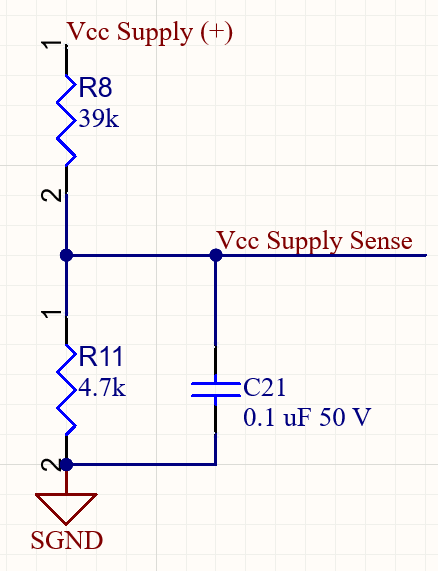
\includegraphics[width=\textwidth]{imagens/voltage_sense.png}
        \caption{Leitura de Tensão.}
        \label{fig:sensor_voltage}
    \end{subfigure}
    \hfill
    \begin{subfigure}[b]{0.32\textwidth}
        \centering
        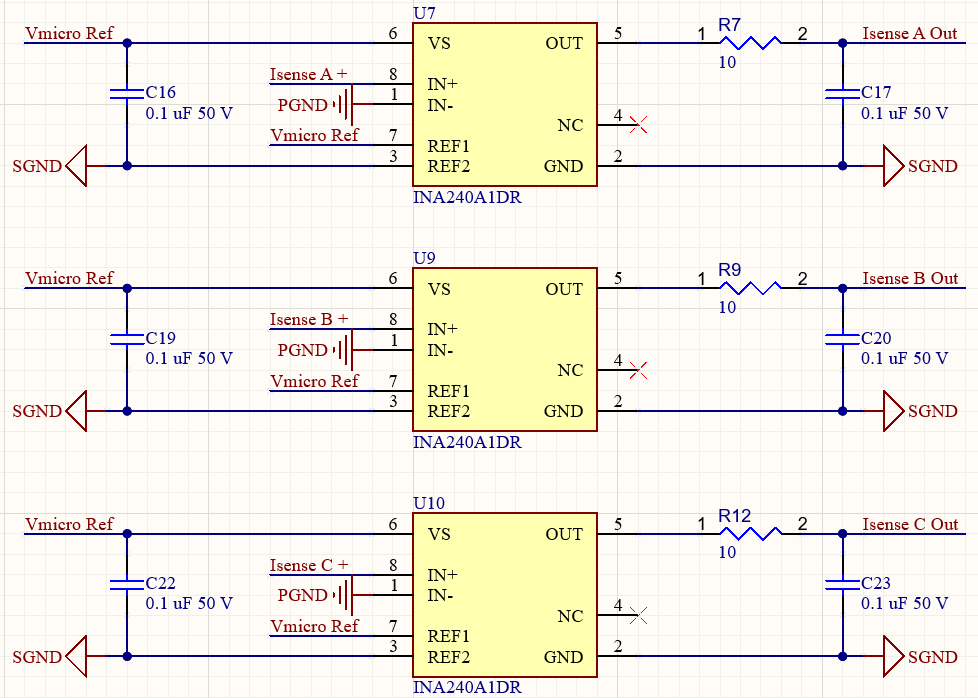
\includegraphics[width=\textwidth]{imagens/current_sense.png}
        \caption{Condicionamento de Corrente.}
        \label{fig:sensor_current}
    \end{subfigure}
    \hfill
    \begin{subfigure}[b]{0.32\textwidth}
        \centering
        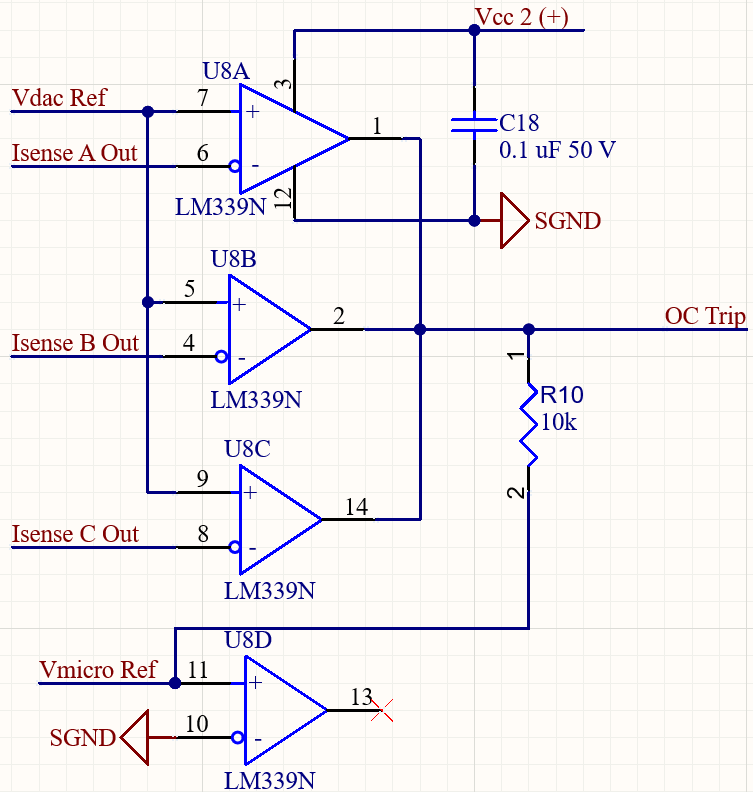
\includegraphics[width=\textwidth]{imagens/ocp_comparator.png}
        \caption{Proteção via \textit{Hardware} (OCP).}
        \label{fig:sensor_ocp}
    \end{subfigure}
    \caption*{Fonte: Elaborado pelo autor.}
\end{figure}

Foi adotado o circuito integrado \textbf{INA240A1DR} em cada fase (Figura \ref{fig:sensor_current}). Este componente é um amplificador de detecção de corrente, projetado especificamente com tecnologia de rejeição de PWM (\textit{Enhanced PWM Rejection}) para suprimir grandes variações de tensão ($dv/dt$) inerentes à comutação de motores. A versão A1DR possui um ganho fixo de $20 \: V/V$. Como as correntes nas bobinas de um motor BLDC são fisicamente alternadas (circulando nos dois sentidos), o microcontrolador seria incapaz de ler o semiciclo negativo, pois seu ADC suporta apenas tensões positivas ($0 \: V$ a $3,3 \: V$). Para viabilizar esta leitura, aplicou-se uma técnica de polarização diferencial: o pino \textit{REF1} foi ligado a $3,3 \: V$ (\textit{Vmicro Ref}) e o pino \textit{REF2} ao \textit{SGND} ($0 \: V$). O circuito do INA240 realiza a média aritmética dessas referências, estabelecendo um \textit{offset} interno exato de $1,65 \: V$ na saída. Consequentemente, uma corrente nula ($0 \: A$) repousa em $1,65 \: V$; correntes positivas elevam a saída em direção a $3,3 \: V$, enquanto correntes negativas a reduzem em direção a $0 \: V$. Este condicionamento garante a bidirecionalidade absoluta da medição, pré-requisito fundamental para a futura implementação de algoritmos avançados de Controle Orientado ao Campo (FOC).

A Figura \ref{fig:sensor_ocp} exibe o circuito de Proteção contra Sobrecorrente (OCP). O \textbf{LM339N} é um circuito integrado que encapsula quatro comparadores de tensão independentes, notável pela sua alta velocidade de reposta (na escala de nanossegundos) e pela sua arquitetura de saída em coletor aberto (\textit{open-collector}). Esta característica de coletor aberto é o que viabiliza a interligação das três proteções de fase em um único nó lógico (\textit{Wired-OR}), utilizando o resistor de \textit{pull-up} R10. Durante a revisão do projeto, realizou-se um ajuste topológico essencial nesta malha: a tensão limitadora (\textit{Vdac Ref}) foi conectada à porta não-inversora (+), enquanto o sinal dos sensores de corrente (\textit{Isense}) foi roteado para a porta inversora (-). Desta forma, em operação nominal ($Isense < Vdac$), os transistores de saída internos do LM339 permanecem em estado de corte (alta impedância), e o R10 mantém o pino \textit{OC Trip} em $3,3 \: V$. No instante em que qualquer fase individual superar o limite de segurança ($Isense > Vdac$), o seu respectivo comparador saturará, conduzindo a linha imediatamente ao terra ($0 \: V$). Esta ação puramente em \textit{hardware} contorna a latência intrínseca de qualquer \textit{software}, gerando uma interrupção prioritária no ESP32 para o bloqueio instantâneo do sinal PWM e salvaguardando a ponte inversora contra catástrofes térmicas ou elétricas.

\pagebreak

\subsection{Estágio de Potência e Ponte Inversora}

A Figura \ref{fig:esquematico_power} expõe a topologia final da ponte inversora trifásica, o núcleo de comutação de força do ESC. O arranjo utiliza seis transistores MOSFET IRFS7530-7PPBF de altíssima capacidade de corrente, estruturados em três braços independentes (Fases A, B e C). Para aumentar a confiabilidade dois detalhes de projeto merecem destaque: a inclusão de resistores de \textit{pull-down} de $10 \: k\Omega$ (R13 a R18) conectados aos terminais \textit{Gate-Source} de cada chave, e a alocação de três resistores \textit{shunt} de liga metálica (encapsulamento de potência 3920, modelo CSS2H-3920R-1L00F de $1 \: m\Omega$) inseridos especificamente nos ramos inferiores da ponte (\textit{Low-Side Sensing}).

\begin{figure}[H]
    \centering
    \caption{Esquemático do estágio de potência contendo a ponte inversora trifásica e resistores \textit{shunt} individuais para medição de corrente.}
    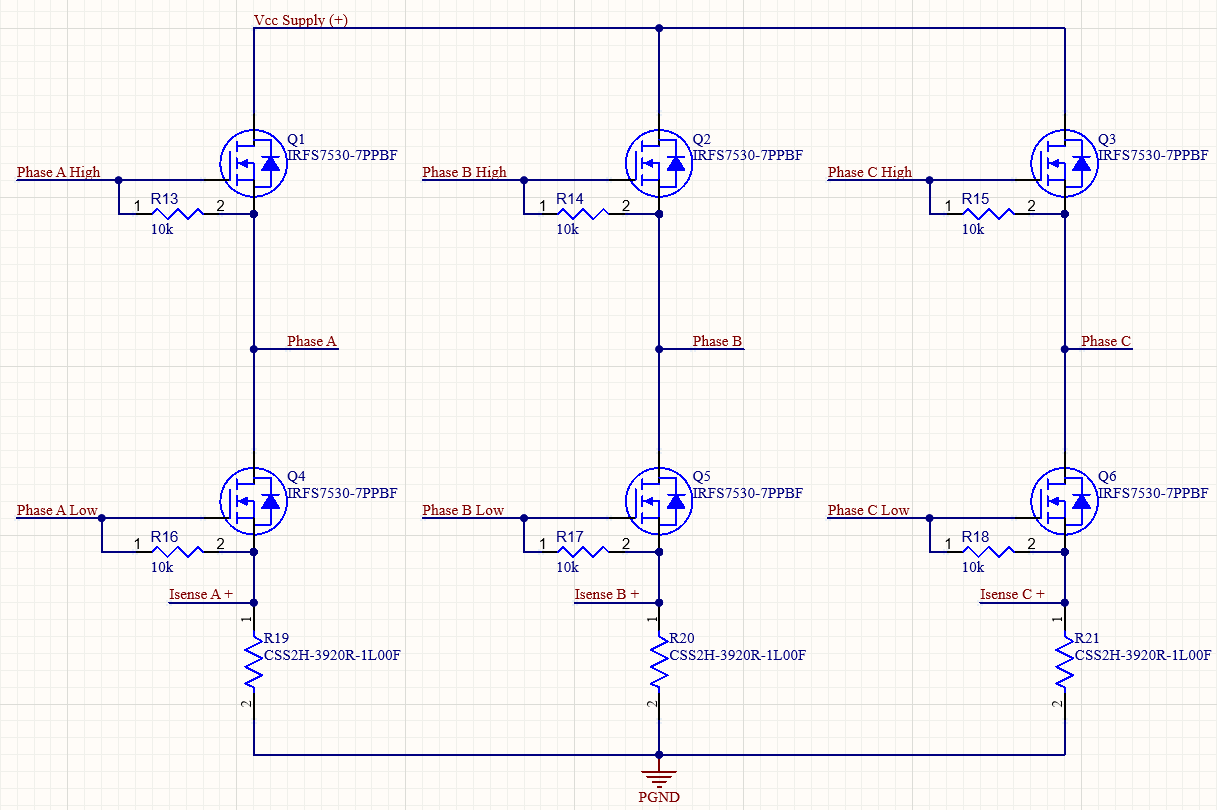
\includegraphics[width=0.9\textwidth]{imagens/esquematico_power.png}
    \caption*{Fonte: Elaborado pelo autor.}
    \label{fig:esquematico_power}
\end{figure}

A função física dos resistores de \textit{pull-down} é garantir um estado seguro de falha (\textit{fail-safe}). Durante a energização inicial do sistema (\textit{power-up}), reinicializações do microcontrolador ou em caso de rompimento físico das trilhas de acionamento, os \textit{gates} dos MOSFETs poderiam assumir um estado flutuante (alta impedância). Nesta condição, ruídos eletromagnéticos acoplados capacitivamente poderiam induzir o acionamento espúrio das chaves, resultando em um curto-circuito catastrófico direto no barramento DC (\textit{shoot-through}). Os resistores de $10 \: k\Omega$ asseguram que a tensão $V_{gs}$ permaneça rigidamente cravada em $0 \: V$ até que os \textit{drivers} IR2110 imponham ativamente o sinal de comando em $15 \: V$. 

Adicionalmente, em relação a escolha do invólucro de 7 pinos para os MOSFETs (D2PAK-7), este encapsulamento possui terminais múltiplos de \textit{Source}, o que minimiza a indutância parasita da pastilha de silício e atenua os anéis de oscilação (\textit{ringing}) durante os transientes de comutação de, no máximo, $90 \: A$. Já a topologia de sensoriamento de corrente no lado baixo (\textit{Low-Side}) atua como uma barreira de proteção para o estágio de condicionamento: em vez de expor os amplificadores INA240 às violentas oscilações de tensão de modo comum (\textit{Common-Mode Voltage}) que variam de $0 \: V$ a $25,2 \: V$ nos nós flutuantes das fases, a medição ocorre de forma referenciada ao terra da placa (\textit{PGND}). A queda de tensão medida sobre o \textit{shunt} de $1 \: m\Omega$ é da ordem de milivolts ($V = R \cdot I$), fornecendo um sinal extremamente limpo, seguro e proporcional à corrente exata que flui para o estator do motor.

\pagebreak

\subsection{Estratégias de Layout, Roteamento e Fabricação da PCB}

O projeto físico do inversor, ilustrado na Figura \ref{fig:pcb_layout}, foi materializado a partir de um laminado virgem de fibra de vidro (FR4) com dupla face de cobre nu, sem a aplicação de máscara de solda comercial (\textit{solder mask}). A placa possui dimensões de $150 \times 200 \: mm$ e espessura de $1,5 \: mm$. Durante a fase de engenharia de manufatura, o método de fabricação sofreu uma alteração: a confecção por corrosão química manual foi substituída pela usinagem em fresadora CNC (\textit{Computer Numerical Control}). A causa física para esta mudança baseia-se na precisão geométrica e na integridade do material condutor. Na corrosão de placas com imensas áreas de cobre, o processo tende a gerar \textit{undercutting} (corrosão lateral) e variações na espessura final da malha. A usinagem CNC atua de forma oposta, removendo mecanicamente apenas o material estritamente necessário para criar os isolamentos (\textit{clearances}), preservando a massa total e a espessura original do cobre contínuo. Para garantir a viabilidade da usinagem, as regras de \textit{design} (DRC) foram ajustadas para manter uma largura mínima de $0,6 \: mm$ nas trilhas de sinais lógicos e um \textit{clearance} mínimo de $0,6 \: mm$ entre elementos, prevenindo curtos-circuitos mecânicos e rompimentos de trilha durante a fresagem.

\begin{figure}[H]
    \centering
    \caption{Projeto de roteamento da Placa de Circuito Impresso no Altium Designer: (a) \textit{Top Layer} evidenciando os polígonos de potência; (b) \textit{Bottom Layer} evidenciando os planos de terra.}
    \label{fig:pcb_layout}
    \begin{subfigure}[b]{0.48\textwidth}
        \centering
        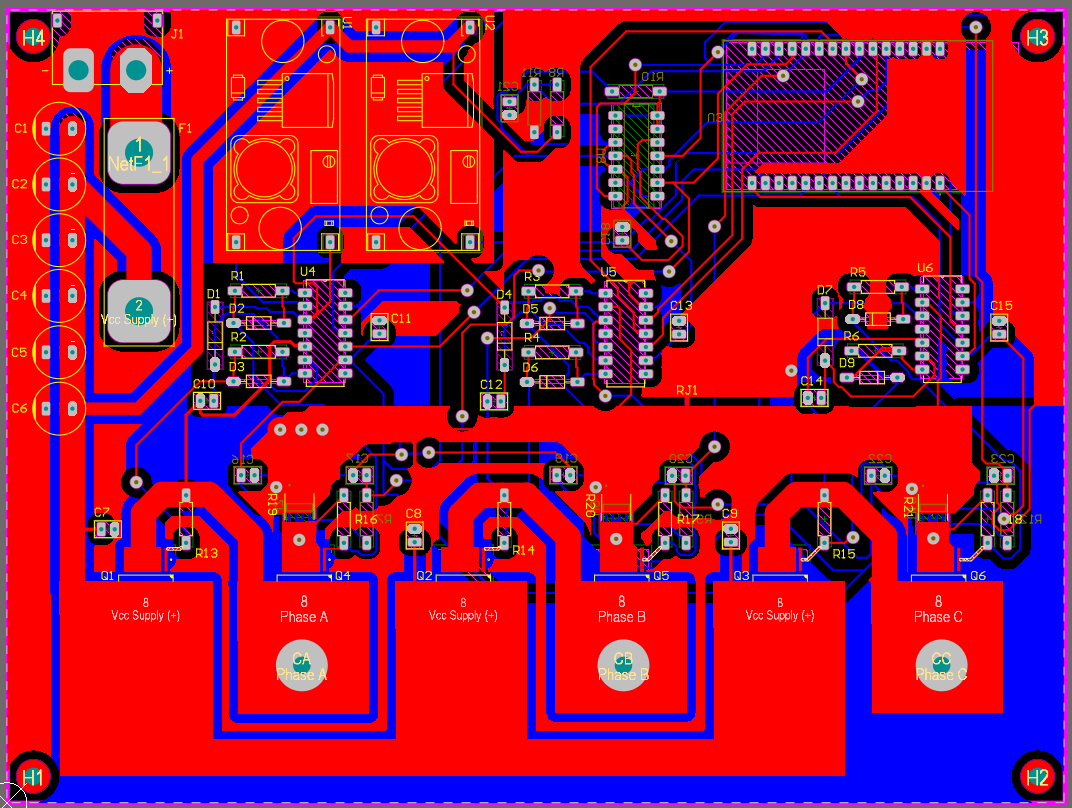
\includegraphics[width=\textwidth]{imagens/pcb_top.png}
        \caption{Camada Superior (\textit{Top Layer}).}
        \label{fig:pcb_top}
    \end{subfigure}
    \hfill
    \begin{subfigure}[b]{0.48\textwidth}
        \centering
        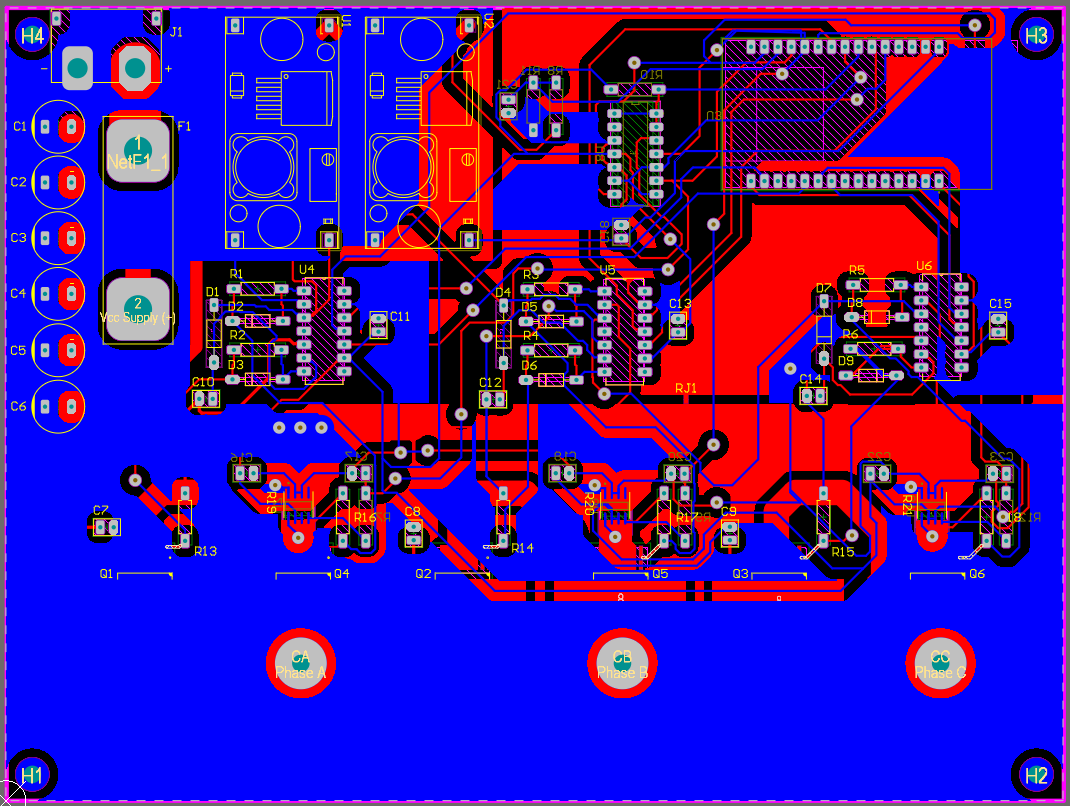
\includegraphics[width=\textwidth]{imagens/pcb_bottom.png}
        \caption{Camada Inferior (\textit{Bottom Layer}).}
        \label{fig:pcb_bottom}
    \end{subfigure}
    \caption*{Fonte: Elaborado pelo autor.}
\end{figure}

Embora as análises computacionais prévias tenham apontado transientes teóricos de comutação com picos próximos a $90 \: A$, ressalta-se que este protótipo inicial de bancada foi projetado para maximizar a capacidade de condução de corrente dentro das limitações físicas de fabricação local, não sendo esperado o regime de operação contínua sob esta magnitude extrema, já que de início o protótipo tem como objetivo demonstrar a viabilidade do design e será testado com um motor e bateria $4S$ e limitado a $3A$. 

Com o propósito de mitigar as perdas ôhmicas, o roteamento físico descartou o uso de trilhas convencionais em favor de grandes polígonos de preenchimento (\textit{copper pours}) sólidos. A camada superior (Figura \ref{fig:pcb_top}) acomoda as ilhas de comutação das fases e o barramento positivo, com gargalos projetados em um mínimo de $5 \: mm$ de largura. Contudo, como a espessura padrão do cobre de um laminado comum (tipicamente $1 \: oz/ft^2$ ou $35 \: \mu m$) possui uma secção transversal insuficiente para conduzir altas correntes, o sistema estaria sujeito à falha por superaquecimento térmico via Efeito Joule ($P = I^2 \cdot R_{trilha}$). Para contornar essa limitação e elevar o limite térmico do circuito, tirou-se proveito da própria natureza do material de prototipagem utilizado: o laminado de cobre nu. A ausência da máscara de solda isolante deixou todos os polígonos de potência naturalmente expostos. Esta característica facilitou a deposição manual de espessas camadas de liga de estanho e o assentamento de condutores de cobre sólido diretamente sobre as malhas críticas, aumentando substancialmente a área da secção transversal ($A$) das trilhas e reduzindo a sua resistência ôhmica equivalente ($\rho \cdot \frac{L}{A}$).

Do ponto de vista de compatibilidade eletromagnética (EMC), duas estratégias de isolamento foram rigorosamente aplicadas no layout. Primeiro, os espaços não roteados da placa foram preenchidos por dois imensos planos de terra funcionalmente segregados: o Terra de Potência (\textit{PGND}), concentrado na camada inferior (Figura \ref{fig:pcb_bottom}) sob o estágio do inversor, e o Terra de Sinal (\textit{SGND}), restrito à periferia dos circuitos lógicos e sensores. A conexão elétrica entre esses dois referenciais foi consolidada estritamente através da técnica de ponto único de aterramento (\textit{Star Ground}). Essa configuração impede o surgimento de laços de terra (\textit{ground loops}) e garante que as severas correntes de retorno induzidas pelo chaveamento do motor permaneçam confinadas na malha de potência, mitigando o fenômeno de flutuação de referencial (\textit{ground bounce}) sobre a eletrônica sensível. Segundo, a Unidade de Controle (ESP32) foi posicionada no extremo oposto da placa em relação aos MOSFETs. Como a comutação rápida de corrente gera campos magnéticos irradiados devido às altas taxas de $di/dt$, o distanciamento físico atua atenuando a intensidade do acoplamento indesejado de forma inversamente proporcional ao quadrado da distância, blindando o microcontrolador contra perturbações eletromagnéticas e travamentos espúrios.
